%% fig4_snr.tex -- generated by fig4_snr.mjs; paste axis envs into main.tex
%% requires only \usepackage{pgfplots} + \usetikzlibrary{arrows.meta}
\begin{figure}[!t]
\centering
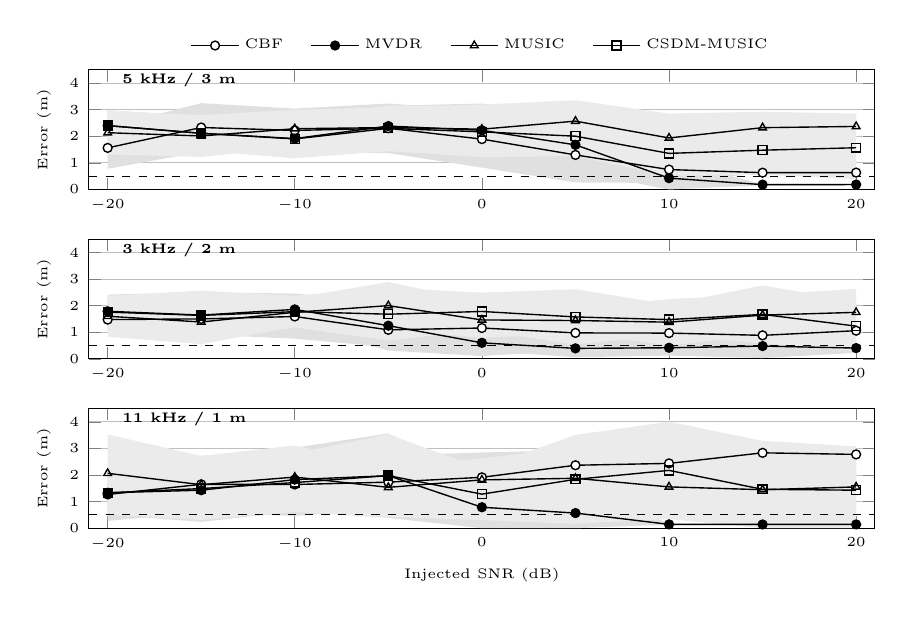
\begin{tikzpicture}[font=\tiny]
\begin{axis}[name=a0, at={(0,0)}, anchor=north west,
  width=\linewidth-16pt, height=3.1cm,
  xmin=-21, xmax=21, ymin=0, ymax=4.5,
  ylabel={Error (m)},
  xtick={-20,-10,0,10,20}, ytick={0,1,2,3,4},
  title={\bfseries 5~kHz / 3~m}, title style={at={(rel axis cs:0.03,0.96)}, anchor=north west, yshift=-2pt},
  legend columns=4, legend style={at={(0.5,1.05)}, anchor=south, draw=none, fill=none, /tikz/every even column/.append style={column sep=8pt}}, legend entries={CBF,MVDR,MUSIC,CSDM-MUSIC},
  ymajorgrids]
\path[fill=black!12] (axis cs:20,0.645) -- (axis cs:15,0.644) -- (axis cs:10,1.252) -- (axis cs:5,2.337) -- (axis cs:0,2.967) -- (axis cs:-5,3.235) -- (axis cs:-10,3.043) -- (axis cs:-15,3.249) -- (axis cs:-20,2.351) -- (axis cs:-20,0.779) -- (axis cs:-15,1.416) -- (axis cs:-10,1.401) -- (axis cs:-5,1.370) -- (axis cs:0,0.823) -- (axis cs:5,0.263) -- (axis cs:10,0.245) -- (axis cs:15,0.620) -- (axis cs:20,0.625) -- cycle;
\path[fill=black!12] (axis cs:20,0.202) -- (axis cs:15,0.208) -- (axis cs:10,1.089) -- (axis cs:5,2.679) -- (axis cs:0,3.235) -- (axis cs:-5,3.149) -- (axis cs:-10,2.642) -- (axis cs:-15,2.760) -- (axis cs:-20,2.975) -- (axis cs:-20,1.831) -- (axis cs:-15,1.468) -- (axis cs:-10,1.189) -- (axis cs:-5,1.622) -- (axis cs:0,1.217) -- (axis cs:5,0.680) -- (axis cs:10,0.000) -- (axis cs:15,0.156) -- (axis cs:20,0.167) -- cycle;
\path[fill=black!8] (axis cs:20,2.855) -- (axis cs:15,2.927) -- (axis cs:10,2.856) -- (axis cs:5,3.358) -- (axis cs:0,3.195) -- (axis cs:-5,3.090) -- (axis cs:-10,2.994) -- (axis cs:-15,2.802) -- (axis cs:-20,2.952) -- (axis cs:-20,1.319) -- (axis cs:-15,1.224) -- (axis cs:-10,1.580) -- (axis cs:-5,1.568) -- (axis cs:0,1.343) -- (axis cs:5,1.785) -- (axis cs:10,1.021) -- (axis cs:15,1.726) -- (axis cs:20,1.888) -- cycle;
\path[fill=black!8] (axis cs:20,2.751) -- (axis cs:15,2.403) -- (axis cs:10,2.200) -- (axis cs:5,2.757) -- (axis cs:0,3.115) -- (axis cs:-5,3.160) -- (axis cs:-10,2.628) -- (axis cs:-15,2.760) -- (axis cs:-20,2.975) -- (axis cs:-20,1.831) -- (axis cs:-15,1.468) -- (axis cs:-10,1.173) -- (axis cs:-5,1.441) -- (axis cs:0,1.222) -- (axis cs:5,1.254) -- (axis cs:10,0.515) -- (axis cs:15,0.552) -- (axis cs:20,0.389) -- cycle;
\addplot[draw=black, mark=*, mark size=1.6pt, mark options={fill=white,draw=black}, line width=0.5pt] coordinates {(20,0.635) (15,0.632) (10,0.749) (5,1.300) (0,1.895) (-5,2.303) (-10,2.222) (-15,2.332) (-20,1.565)};
\addplot[draw=black, mark=*, mark size=1.6pt, mark options={fill=black,draw=black}, line width=0.5pt] coordinates {(20,0.185) (15,0.182) (10,0.426) (5,1.679) (0,2.226) (-5,2.386) (-10,1.915) (-15,2.114) (-20,2.403)};
\addplot[draw=black, mark=triangle, mark size=1.6pt, mark options={fill=gray!25,draw=black}, line width=0.5pt] coordinates {(20,2.372) (15,2.326) (10,1.938) (5,2.572) (0,2.269) (-5,2.329) (-10,2.287) (-15,2.013) (-20,2.136)};
\addplot[draw=black, mark=square, mark size=1.6pt, mark options={fill=gray!60,draw=black}, line width=0.5pt] coordinates {(20,1.570) (15,1.478) (10,1.358) (5,2.005) (0,2.168) (-5,2.300) (-10,1.901) (-15,2.114) (-20,2.403)};
\draw[dashed] (axis cs:-21,0.5) -- (axis cs:21,0.5);
\end{axis}
\begin{axis}[name=a1, at={(a0.south)}, anchor=north, yshift=-18pt,
  width=\linewidth-16pt, height=3.1cm,
  xmin=-21, xmax=21, ymin=0, ymax=4.5,
  ylabel={Error (m)},
  xtick={-20,-10,0,10,20}, ytick={0,1,2,3,4},
  title={\bfseries 3~kHz / 2~m}, title style={at={(rel axis cs:0.03,0.96)}, anchor=north west, yshift=-2pt},
  ymajorgrids]
\path[fill=black!12] (axis cs:20,1.894) -- (axis cs:15,1.739) -- (axis cs:10,1.816) -- (axis cs:5,1.893) -- (axis cs:0,2.015) -- (axis cs:-5,1.743) -- (axis cs:-10,2.428) -- (axis cs:-15,2.087) -- (axis cs:-20,1.938) -- (axis cs:-20,1.016) -- (axis cs:-15,0.918) -- (axis cs:-10,0.758) -- (axis cs:-5,0.441) -- (axis cs:0,0.304) -- (axis cs:5,0.059) -- (axis cs:10,0.123) -- (axis cs:15,0.029) -- (axis cs:20,0.225) -- cycle;
\path[fill=black!12] (axis cs:20,0.475) -- (axis cs:15,0.854) -- (axis cs:10,0.495) -- (axis cs:5,0.463) -- (axis cs:0,1.099) -- (axis cs:-5,2.183) -- (axis cs:-10,2.457) -- (axis cs:-15,2.504) -- (axis cs:-20,2.419) -- (axis cs:-20,1.161) -- (axis cs:-15,0.789) -- (axis cs:-10,1.264) -- (axis cs:-5,0.312) -- (axis cs:0,0.105) -- (axis cs:5,0.326) -- (axis cs:10,0.339) -- (axis cs:15,0.106) -- (axis cs:20,0.334) -- cycle;
\path[fill=black!8] (axis cs:20,2.634) -- (axis cs:15,2.414) -- (axis cs:10,2.249) -- (axis cs:5,1.914) -- (axis cs:0,2.138) -- (axis cs:-5,2.891) -- (axis cs:-10,2.293) -- (axis cs:-15,2.222) -- (axis cs:-20,2.375) -- (axis cs:-20,0.831) -- (axis cs:-15,0.551) -- (axis cs:-10,1.212) -- (axis cs:-5,1.115) -- (axis cs:0,0.790) -- (axis cs:5,0.971) -- (axis cs:10,0.511) -- (axis cs:15,0.876) -- (axis cs:20,0.865) -- cycle;
\path[fill=black!8] (axis cs:20,2.160) -- (axis cs:15,2.764) -- (axis cs:10,2.049) -- (axis cs:5,2.620) -- (axis cs:0,2.493) -- (axis cs:-5,2.670) -- (axis cs:-10,2.372) -- (axis cs:-15,2.568) -- (axis cs:-20,2.369) -- (axis cs:-20,1.150) -- (axis cs:-15,0.701) -- (axis cs:-10,1.180) -- (axis cs:-5,0.690) -- (axis cs:0,1.073) -- (axis cs:5,0.534) -- (axis cs:10,0.905) -- (axis cs:15,0.583) -- (axis cs:20,0.302) -- cycle;
\addplot[draw=black, mark=*, mark size=1.6pt, mark options={fill=white,draw=black}, line width=0.5pt] coordinates {(20,1.060) (15,0.884) (10,0.969) (5,0.976) (0,1.160) (-5,1.092) (-10,1.593) (-15,1.503) (-20,1.477)};
\addplot[draw=black, mark=*, mark size=1.6pt, mark options={fill=black,draw=black}, line width=0.5pt] coordinates {(20,0.405) (15,0.480) (10,0.417) (5,0.394) (0,0.602) (-5,1.248) (-10,1.861) (-15,1.646) (-20,1.790)};
\addplot[draw=black, mark=triangle, mark size=1.6pt, mark options={fill=gray!25,draw=black}, line width=0.5pt] coordinates {(20,1.750) (15,1.645) (10,1.380) (5,1.442) (0,1.464) (-5,2.003) (-10,1.752) (-15,1.386) (-20,1.603)};
\addplot[draw=black, mark=square, mark size=1.6pt, mark options={fill=gray!60,draw=black}, line width=0.5pt] coordinates {(20,1.231) (15,1.673) (10,1.477) (5,1.577) (0,1.783) (-5,1.680) (-10,1.776) (-15,1.635) (-20,1.760)};
\draw[dashed] (axis cs:-21,0.5) -- (axis cs:21,0.5);
\end{axis}
\begin{axis}[name=a2, at={(a1.south)}, anchor=north, yshift=-18pt,
  width=\linewidth-16pt, height=3.1cm,
  xmin=-21, xmax=21, ymin=0, ymax=4.5,
  xlabel={Injected SNR (dB)}, ylabel={Error (m)},
  xtick={-20,-10,0,10,20}, ytick={0,1,2,3,4},
  title={\bfseries 11~kHz / 1~m}, title style={at={(rel axis cs:0.03,0.96)}, anchor=north west, yshift=-2pt},
  ymajorgrids]
\path[fill=black!12] (axis cs:20,3.034) -- (axis cs:15,2.839) -- (axis cs:10,3.076) -- (axis cs:5,2.940) -- (axis cs:0,2.851) -- (axis cs:-5,2.732) -- (axis cs:-10,2.828) -- (axis cs:-15,2.725) -- (axis cs:-20,2.264) -- (axis cs:-20,0.277) -- (axis cs:-15,0.579) -- (axis cs:-10,0.462) -- (axis cs:-5,0.736) -- (axis cs:0,0.982) -- (axis cs:5,1.800) -- (axis cs:10,1.804) -- (axis cs:15,2.834) -- (axis cs:20,2.522) -- cycle;
\path[fill=black!12] (axis cs:20,0.142) -- (axis cs:15,0.142) -- (axis cs:10,0.153) -- (axis cs:5,1.852) -- (axis cs:0,1.897) -- (axis cs:-5,3.564) -- (axis cs:-10,3.030) -- (axis cs:-15,2.622) -- (axis cs:-20,2.158) -- (axis cs:-20,0.508) -- (axis cs:-15,0.238) -- (axis cs:-10,0.628) -- (axis cs:-5,0.389) -- (axis cs:0,0.000) -- (axis cs:5,0.000) -- (axis cs:10,0.136) -- (axis cs:15,0.142) -- (axis cs:20,0.142) -- cycle;
\path[fill=black!8] (axis cs:20,2.518) -- (axis cs:15,2.294) -- (axis cs:10,2.381) -- (axis cs:5,3.047) -- (axis cs:0,2.625) -- (axis cs:-5,2.329) -- (axis cs:-10,3.117) -- (axis cs:-15,2.721) -- (axis cs:-20,3.528) -- (axis cs:-20,0.604) -- (axis cs:-15,0.555) -- (axis cs:-10,0.733) -- (axis cs:-5,0.746) -- (axis cs:0,1.012) -- (axis cs:5,0.711) -- (axis cs:10,0.728) -- (axis cs:15,0.603) -- (axis cs:20,0.589) -- cycle;
\path[fill=black!8] (axis cs:20,3.079) -- (axis cs:15,3.288) -- (axis cs:10,4.009) -- (axis cs:5,3.511) -- (axis cs:0,2.258) -- (axis cs:-5,3.533) -- (axis cs:-10,2.823) -- (axis cs:-15,2.670) -- (axis cs:-20,2.158) -- (axis cs:-20,0.508) -- (axis cs:-15,0.313) -- (axis cs:-10,0.612) -- (axis cs:-5,0.427) -- (axis cs:0,0.306) -- (axis cs:5,0.167) -- (axis cs:10,0.343) -- (axis cs:15,0.000) -- (axis cs:20,0.000) -- cycle;
\addplot[draw=black, mark=*, mark size=1.6pt, mark options={fill=white,draw=black}, line width=0.5pt] coordinates {(20,2.778) (15,2.837) (10,2.440) (5,2.370) (0,1.916) (-5,1.734) (-10,1.645) (-15,1.652) (-20,1.270)};
\addplot[draw=black, mark=*, mark size=1.6pt, mark options={fill=black,draw=black}, line width=0.5pt] coordinates {(20,0.142) (15,0.142) (10,0.144) (5,0.570) (0,0.789) (-5,1.977) (-10,1.829) (-15,1.430) (-20,1.333)};
\addplot[draw=black, mark=triangle, mark size=1.6pt, mark options={fill=gray!25,draw=black}, line width=0.5pt] coordinates {(20,1.554) (15,1.449) (10,1.555) (5,1.879) (0,1.819) (-5,1.538) (-10,1.925) (-15,1.638) (-20,2.066)};
\addplot[draw=black, mark=square, mark size=1.6pt, mark options={fill=gray!60,draw=black}, line width=0.5pt] coordinates {(20,1.431) (15,1.464) (10,2.176) (5,1.839) (0,1.282) (-5,1.980) (-10,1.718) (-15,1.492) (-20,1.333)};
\draw[dashed] (axis cs:-21,0.5) -- (axis cs:21,0.5);
\end{axis}
\end{tikzpicture}
\caption{Mean localization error (over 20 projector events, $\pm$1 std shaded)
versus injected band-matched noise SNR for the four algorithms in three
projector conditions (post-processing injection on the original 8-channel
recordings; dashed: 0.5~m failure threshold).}
\label{fig:snr}
\end{figure}
